\documentclass[12pt]{article}
\usepackage[top=5mm,includehead,headheight=63pt, left=2.5cm,bottom=2.5cm,right=2.5cm,headsep=0.3cm]{geometry} 
\usepackage{fontspec}
\setmainfont[
 Path = fonts/,
 BoldFont={Veleka-Bold.otf}, 
 ItalicFont={Veleka-Italic.otf},
 BoldItalicFont={Veleka-BoldItalic.otf}
 ]{Veleka-Regular.otf}


%% bibliography packages
\usepackage{biblatex} 
\addbibresource{biblo.bib} 

%%charset packages
\usepackage[utf8]{inputenc}
\usepackage[english,bulgarian]{babel}
\usepackage{textgreek}
\usepackage{textcomp}
\usepackage[T2A]{fontenc}

%% hyperlinks
\usepackage{hyperref}
\usepackage{url}[hyphens]

%% graphics packages
\usepackage{caption}
\usepackage{graphicx}
\usepackage{subfigure}
\graphicspath{{imgs/}}
\usepackage{float}




%%Autoref language settings begin
\renewcommand*{\figureautorefname}{Фиг.}
\renewcommand*{\equationautorefname}{Уравн.}
\renewcommand*{\subsectionautorefname}{Пар.}
\renewcommand*{\subsubsectionautorefname}{\subsectionautorefname}
\newcommand{\subfigureautorefname}{\figureautorefname}
%%Autoref language settings end

%%other
\usepackage[inline]{enumitem}
\usepackage{amsmath}
\usepackage{amssymb}
\usepackage{breqn}
\allowdisplaybreaks
\usepackage{fancyhdr}
\usepackage{afterpage}
\usepackage{listings}
\lstloadlanguages{[5.2]Mathematica}


\title{Математически модел на идеален контакт}
\author{Васил Иванов}
\date{\today}

%%header definitions
\pagestyle{fancy}
\fancyhf{}
\lhead{
\includegraphics[width=0.1\linewidth]{su-logo.png}}
\chead{СОФИЙСКИ УНИВЕРСИТЕТ „Св. КЛИМЕНТ ОХРИДСКИ”\\Факултет по химия и фармация}
\fancyfoot[C]{\ifnum\thepage<2\relax\else\thepage\fi}
%%end header definitions

\begin{document}
\begin{titlepage}
    \thispagestyle{fancy}
    \begin{center}
        \hfill \break
        \hfill \break
        \hfill \break
        \Huge	
        \textbf{Курсова работа}\\
        \vspace{3cm}
    \end{center}
    \normalsize	
    \textbf{\underline{Тема:}} Модел на идеален топлинен контакт
    \vspace{2cm}

    \begin{flushright}
        \normalsize	
        Изготвил: Васил Василев Иванов,

        Магистърска програма: ,,Изчислителна математика и математическо моделиране``
        \vspace{1cm}

        За курса:

        ,,Математически модели и изчислитен експеримент``
    \end{flushright}

    \vspace*{\fill}
    \begin{center}
        \footnotesize	
        София

         ~2022~г.
    \end{center}
 \end{titlepage}
\setcounter{page}{2}

\section{Задача}
Разглеждаме задачата за идеален топлинен контакт:
\begin{align}
	\frac{\partial u_1}{\partial t} & = \kappa_{1}  \frac{\partial ^ 2 u_1}{\partial x ^ 2}, - \infty < x < 0; 0 < t \leq T \\ 
	\frac{\partial u_2}{\partial t} & = \kappa_{2}  \frac{\partial ^ 2 u_2}{\partial x ^ 2}, 0 < x < \infty; 0 < t \leq T   
\end{align}
Където:
\begin{equation}
	\kappa_{i} = \frac{k_{i}}{\rho_{i} c_{i}}
\end{equation}

\begin{itemize}
	\item $\kappa_{i}$ - температуропроводност
	\item $k_{i}$ - топлопроводност
	\item $c_{i}$ - топлинен капацитет
	\item $\rho_{i}$  - плътност на материала
\end{itemize}

Наложено е и следното прекъснато начално условие
\begin{align}
	u_{1}(x, t = 0) & = 0, -\infty < x < 0  \\
	u_{2}(x, t = 0) & = u_0, 0 < x < \infty 
\end{align}

Както и гранични условия ,,на безкрайност``:
\begin{align}
	u_{1}(-\infty, t) & = 0, t > 0   \\
	u_{2}(+\infty, t) & = u_0, t > 0 
\end{align}
 
И условията за идеален контакт:
\begin{align}
	u_{1}(0, t)                                 & = u_2(0, t),  t > 0                                  \\
	k_{1}\frac{\partial u_1}{\partial x} (0, t) & = k_{2}\frac{\partial u_2}{\partial x} (0, t), t > 0 
\end{align}

Дефинираме и ,,помощна константа`` $\beta$ с цел олекотяване на записа:
\begin{equation*}
	\beta = \frac{\sqrt{k_2 \rho_2 c_2}}{\sqrt{k_1 \rho_1 c_1}}
\end{equation*}

За така поставената задача е известно и точното (аналитично решение):
\begin{align}
	u_{1}(x, t) & = \frac{\beta u_0}{1+\beta} \left[1 + \erf{\left(\frac{2}{2\sqrt{\kappa_1 t}}\right)}\right] \\
	u_{2}(x, t) & = \frac{u_0}{1+\beta} \left[\beta + \erf{\left(\frac{2}{2\sqrt{\kappa_2 t}}\right)}\right]   
\end{align}
Където: 
\begin{equation*}
	\erf{(z)} = \frac{2}{\sqrt{\pi}} \displaystyle\int_{0}^{z} e ^{-t^2} dt
\end{equation*}
За целите на изследването на полученото числено решение ще използваме следните физични пареметри за различни материали:\\
\begin{figure}[h]
	\centering
	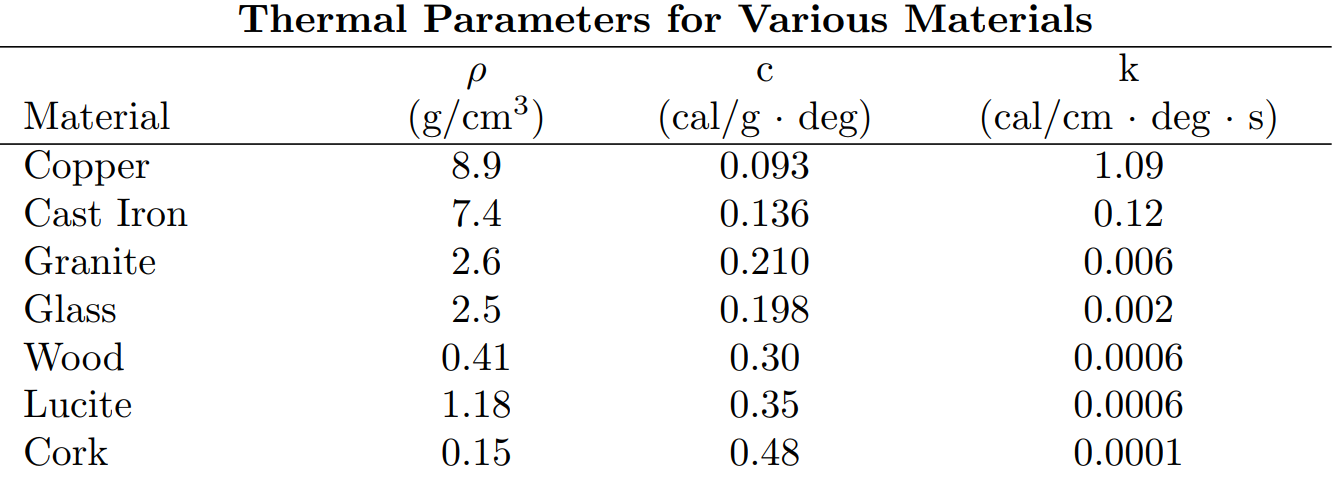
\includegraphics[width=\linewidth]{constants.png}
	\caption{Термофизични константи за различни материали}
	\label{fig:constants}
\end{figure}

\end{document}
